%
\documentclass{standalone}
% \usepackage{tikz}
\usepackage{pgfplots} % loads also tikz
\usepackage{grffile}
\pgfplotsset{compat=newest} % This will configure the compatibility layer
\usetikzlibrary{plotmarks}
\usepackage{amsmath}
\usepackage{color} % Using this package, you can set the font color, text background, or page background
\usetikzlibrary{arrows,shapes,positioning}
\usepackage{anyfontsize}
\usepackage{siunitx}

\tikzset{ % Set line width
	ultra thin/.style= {line width=0.1pt},
	very thin/.style=  {line width=0.2pt},
	thin/.style=       {line width=0.4pt},% thin is the default
	semithick/.style=  {line width=0.6pt},
	thick/.style=      {line width=0.8pt},
	very thick/.style= {line width=1.2pt},
	ultra thick/.style={line width=1.6pt}
}

% Defines color spec 
% http://www.color-hex.com for color details

\definecolor{vancolor}{HTML}{1c375b}  
\definecolor{vbncolor}{HTML}{5b1c37}
\definecolor{vcncolor}{HTML}{375b1c}
\definecolor{vabcolor}{HTML}{5b401c}
\definecolor{vbccolor}{HTML}{1c5b40}
\definecolor{vcacolor}{HTML}{401c5b}
\definecolor{vbacolor}{HTML}{FF0080}
\definecolor{vcbcolor}{HTML}{FF0000}
\definecolor{vaccolor}{HTML}{800000}



%\definecolor{vancolor}{HTML}{000000} 
%\definecolor{vbncolor}{HTML}{202120}
%\definecolor{vcncolor}{HTML}{363735}
%\definecolor{vabcolor}{HTML}{4b4d4a}
%\definecolor{vbccolor}{HTML}{4c4c4c}
%\definecolor{vcacolor}{HTML}{595959}
%\definecolor{vbacolor}{HTML}{666666}
%\definecolor{vcbcolor}{HTML}{666666}
%\definecolor{vaccolor}{HTML}{474747}


% Define a espessura da linha
\def \vanlw {thin}
\def \vbnlw {thin}
\def \vcnlw {thin}
\def \vablw {ultra thick}
\def \vbclw {ultra thick}
\def \vcalw {ultra thick}
\def \vbalw {thin}
\def \vcblw {thin}
\def \vaclw {thin}


% Definitions
\def\refdist{2.5mm} % Channel ref arrow length
\def\tipangleA{125} % Tip angle for CH1
\def\tipangleB{125} % Tip angle for CH2
\def\tipangleC{-45} % Tip angle for CH3
\def\tipangleD{75} % Tip angle for CH4
\def\tipangleE{75} % Tip angle for CH5
\def\tipdist{5mm} % Tip arrow legth

% Defines axis aspect ratio
\def \axisheight {\linewidth}
\def \axiswidth {1.4\linewidth} 

\def \alphathy {0.5235} 

\pgfplotsset{Axis Style/.style={
		width=\axiswidth , height=\axisheight,
		axis x line=center,
		axis y line=middle,
		samples=200,
		ymin=-1.732, ymax=1.732,
		xmin=0, xmax=13.5,
		domain=0:4*pi,
	}}
	

\begin{document}
	\fontsize{8}{10}\selectfont
 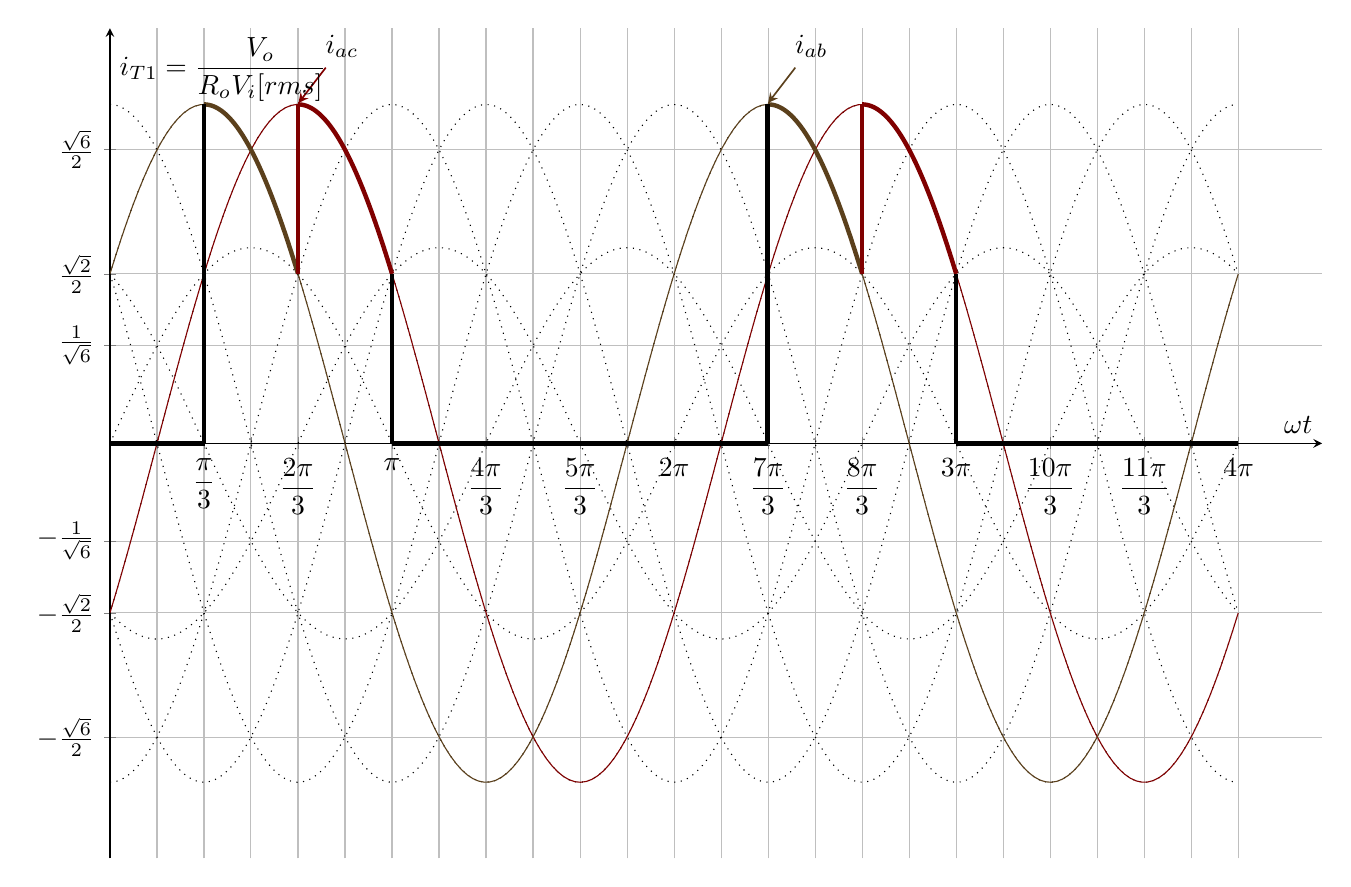
\begin{tikzpicture}   
\begin{axis}[
Axis Style,
grid=major,
xtick={	0,0.5236, 1.0472, 1.57, 2.0944,2.618, 3.1416, 3.665, 4.188, 4.712,5.236, 5.76, 6.28318, 6.8068, 7.33, 7.854, 8.377, 8.901, 9.4248, 9.948, 10.472, 11,11.52, 12.043, 12.57 },
xticklabels={
	$0$, , $\dfrac{\pi}{3}$, ,$\dfrac{2\pi}{3}$, ,$\pi$, ,$\dfrac{4\pi}{3}$, , $\dfrac{5\pi}{3}$, , $2\pi$, , $\dfrac{7\pi}{3}$, ,$\dfrac{8\pi}{3}$, ,$3\pi$, ,$\dfrac{10\pi}{3}$, ,$\dfrac{11\pi}{3}$, ,$4\pi$},
%xticklabels={
%	$0$,$\dfrac{\pi}{6}$ , $\dfrac{\pi}{3}$,$\dfrac{\pi}{2}$ ,$\dfrac{2\pi}{3}$,$\dfrac{5\pi}{6}$ ,$\pi$,$\dfrac{7\pi}{6}$ ,$\dfrac{4\pi}{3}$, $\dfrac{3\pi}{2}$, $\dfrac{5\pi}{3}$,$\dfrac{11\pi}{6}$ , $2\pi$, $\dfrac{13\pi}{6}$, $\dfrac{7\pi}{3}$, $\dfrac{5\pi}{2}$ ,$\dfrac{8\pi}{3}$, $\dfrac{17\pi}{6}$ ,$3\pi$,$\dfrac{19\pi}{6}$ ,$\dfrac{10\pi}{3}$,$\dfrac{7\pi}{2}$ ,$\dfrac{11\pi}{3}$, $\dfrac{23\pi}{6}$ ,$4\pi$},
%xticklabels={
%	$0$,$\dfrac{\pi}{6}$ , ,$\dfrac{\pi}{2}$ ,,$\dfrac{5\pi}{6}$ ,,$\dfrac{7\pi}{6}$ ,, $\dfrac{3\pi}{2}$, ,$\dfrac{11\pi}{6}$ , , $\dfrac{13\pi}{6}$, , $\dfrac{5\pi}{2}$ ,, $\dfrac{17\pi}{6}$ ,,$\dfrac{19\pi}{6}$ ,,$\dfrac{7\pi}{2}$ ,, $\dfrac{23\pi}{6}$ ,},
ytick={-1.226,-0.7071,-0.4082,0,0.4082, 0.7071, 1.225},
yticklabels={$-\frac{\sqrt{6}}{2}$,$-\frac{\sqrt{2}}{2}$,$-\frac{1}{\sqrt{6}}$,$0$,$\frac{1}{\sqrt{6}}$,$\frac{\sqrt{2}}{2}$,$\frac{\sqrt{6}}{2}$},
ylabel={$i_{T1}=\dfrac{V_{o}}{R_oV_{i}[rms]}$},
xlabel={$\omega t$},
]

\addplot [mark=none,dotted] {sqrt(2/3)*sin(deg(x))};  % Van
\addplot [mark=none,dotted] {sqrt(2/3)*sin(deg(x-2.0944))};  % Vbn
\addplot [mark=none,dotted] {sqrt(2/3)*sin(deg(x+2.0944))};  % Vcn


\addplot [mark=none,dotted] {sqrt(2)*sin(deg(x+(11*3.1415/6)))}; % Vab
\addplot [mark=none,dotted] {-sqrt(2)*sin(deg(x+(11*3.1415/6)))}; % Vba
\addplot [mark=none,dotted] {sqrt(2)*cos(deg(x))}; % Vbc
\addplot [mark=none,dotted] {-sqrt(2)*cos(deg(x))}; % Vcb
\addplot [mark=none,dotted] {sqrt(2)*sin(deg(x+(7*3.1415/6)))}; % Vca
\addplot [mark=none,dotted] {-sqrt(2)*sin(deg(x+(7*3.1415/6)))}; % Vac



%
%\addplot [mark=none, vancolor,ultra thick] {sqrt(2/3)*sin(deg(x))};  % Van
%\addplot [mark=none, vcncolor,ultra thick] {sqrt(2/3)*sin(deg(x+2.0944))};  % Vcn
%\addplot [mark=none, vbncolor,ultra thick] {sqrt(2/3)*sin(deg(x-2.0944))};  % Vbn%

%[domain=0:pi/6] -- [domain=pi/6:pi]
\addplot [mark=none, vaccolor,ultra thick][domain=pi/2+\alphathy:5*pi/6+\alphathy]{sqrt(2)*sin(deg(x+(11*3.1415/6)))}; % Vac
%\addplot [mark=none, vcacolor,ultra thick]{-sqrt(2)*sin(deg(x+(11*3.1415/6)))}; % Vca
\addplot [mark=none, vaccolor]{sqrt(2)*sin(deg(x+(11*3.1415/6)))}; % Vac

\addplot [mark=none, vaccolor,ultra thick][domain=5*pi/2+\alphathy:17*pi/6+\alphathy]{sqrt(2)*sin(deg(x+(11*3.1415/6)))}; % Vac




%\addplot [mark=none, vcbcolor,ultra thick] {sqrt(2)*cos(deg(x))}; % Vcb
%\addplot [mark=none, vbccolor,ultra thick] {-sqrt(2)*cos(deg(x))}; % Vbc

%\addplot [mark=none, vbacolor,ultra thick] {sqrt(2)*sin(deg(x+(7*3.1415/6)))}; % Vba
\addplot [mark=none, vabcolor,ultra thick][domain=pi/6+\alphathy:pi/2+\alphathy]{-sqrt(2)*sin(deg(x+(7*3.1415/6)))}; % Vab
\addplot [mark=none, vabcolor,ultra thick][domain=13*pi/6+\alphathy:5*pi/2+\alphathy]{-sqrt(2)*sin(deg(x+(7*3.1415/6)))}; % Vab

\addplot [mark=none, vabcolor]{-sqrt(2)*sin(deg(x+(7*3.1415/6)))}; % Vab

%
\addplot [mark=none, black,ultra thick][domain=0:pi/6+\alphathy]{0}; % Vca
\addplot [mark=none, black,ultra thick][domain=5*pi/6+\alphathy:13*pi/6+\alphathy]{0}; % Vca
\addplot [mark=none, black,ultra thick][domain=17*pi/6+\alphathy:4*pi]{0}; % Vca


%
\draw[mark=none, black,ultra thick] (axis cs:0.523+\alphathy,0) -- (axis cs:0.523+\alphathy,1.4142);
\draw[mark=none, black,ultra thick] (axis cs:2.62+\alphathy,0) -- (axis cs:2.62+\alphathy,0.707);
\draw[mark=none, black,ultra thick] (axis cs:6.8+\alphathy,0) -- (axis cs:6.8+\alphathy,1.4142);
\draw[mark=none, black,ultra thick] (axis cs:8.9+\alphathy,0) -- (axis cs:8.9+\alphathy,0.707);

\draw[mark=none, vaccolor,ultra thick] (axis cs:1.57+\alphathy,0.707) -- (axis cs:1.57+\alphathy,1.4142);
\draw[mark=none, vaccolor,ultra thick] (axis cs:7.85+\alphathy,0.707) -- (axis cs:7.85+\alphathy,1.4142);

% Indicadores 
%\node[coordinate,pin={[pin distance=\tipdist,pin edge={stealth-,semithick,vancolor}]64:{$v_{an}$}}] at (axis cs:1.57,0.83){}; % Print curve tip
%\node[coordinate,pin={[pin distance=\tipdist,pin edge={stealth-,semithick,vcncolor}]64:{$v_{cn}$}}] at (axis cs:5.76,0.83){}; % Print curve tip
%\node[coordinate,pin={[pin distance=\tipdist,pin edge={stealth-,semithick,vbncolor}]64:{$v_{bn}$}}] at (axis cs:3.67,0.83){}; % Print curve tip


\node[coordinate,pin={[pin distance=\tipdist,pin edge={stealth-,semithick,vaccolor}]64:{$i_{ac}$}}] at (axis cs:2.1,1.42){}; % Print curve tip
%\node[coordinate,pin={[pin distance=\tipdist,pin edge={stealth-,semithick,vcacolor}]64:{$v_{ca}$}}] at (axis cs:5.24,1.42){}; % Print curve tip

%\node[coordinate,pin={[pin distance=\tipdist,pin edge={stealth-,semithick,vcbcolor}]64:{$v_{cb}$}}] at (axis cs:6.28,1.42){}; % Print curve tip
%\node[coordinate,pin={[pin distance=\tipdist,pin edge={stealth-,semithick,vbccolor}]64:{$v_{bc}$}}] at (axis cs:3.14,1.42){}; % Print curve tip


%\node[coordinate,pin={[pin distance=\tipdist,pin edge={stealth-,semithick,vabcolor}]64:{$v_{ba}$}}] at (axis cs:4.188,1.42){}; % Print curve tip
\node[coordinate,pin={[pin distance=\tipdist,pin edge={stealth-,semithick,vabcolor}]64:{$i_{ab}$}}] at (axis cs:7.33,1.42){}; % Print curve tip


\end{axis}
        
    \end{tikzpicture}
    
    
\end{document} % End of file